\section{Problem Definition -- Big Picture}
\label{sec:definition}

Loosely speaking, the high-level objective in transient-detection is to locate intrinsically(?)-varying objects in each recently shot image of the sky.
More formally and in the concept of this project, this objective can be defined as finding the mapping
\begin{equation}
  \label{eq:def1}
  (I_t,I_s) \longrightarrow S_t 
\end{equation}
where $I_s$ is the recently captured image, namely the \emph{science image}. $I_t$ is the \emph{template} or \emph{reference} image, and $S_t$ is the set of \emph{true transients} to be detected.


However, this problem has traditionally been broken down into two broad sub-problems, namely, \emph{image differencing}\footnote{or interchangeably, \emph{difference imaging}} and \emph{smart-thresholding}; the latter being the process of finding a threshold above which all the pixels in the diff image, $I_d$, will be seen as candidate transient sources:
\begin{equation}
  \label{eq:def2}
  (I_t,I_s) \xrightarrow{diff} I_d \xrightarrow{threshold} S_t 
\end{equation}

\begin{figure}[h]
  \centering
  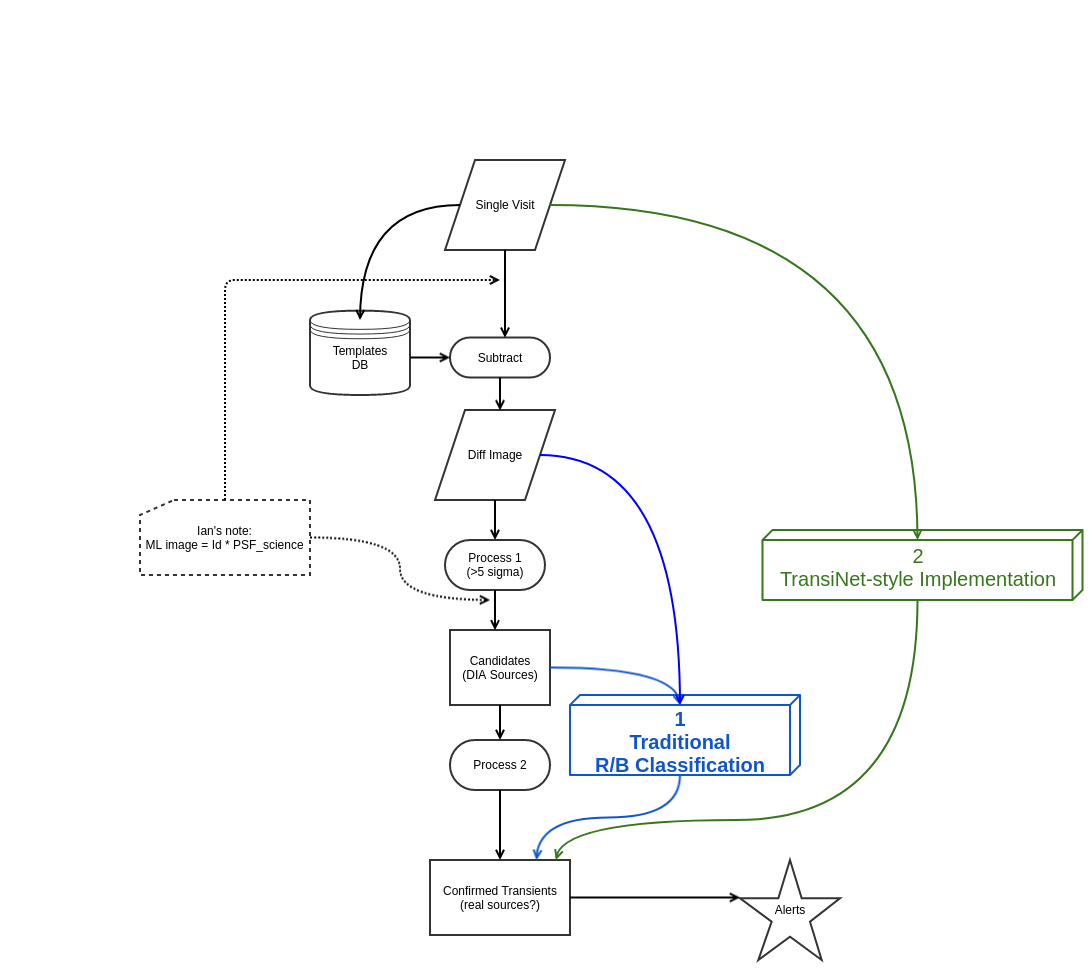
\includegraphics[width=.8\textwidth]{material/diagram}
  \caption{Coarse illustration of information flow through the Alert Production (AP) pipeline. Paths in blue and green illustrate the ``traditional'' and ``modern'' approaches respectively.}
  \label{fig:diagram}
\end{figure}


The \emph{thresholding} step has traditionally been implemented as a simple $5\sigma$-thresholding, but other auxiliary approaches, such as pre-convolution with the PSF, may wrap around this stage to make it smart -- figure~\ref{fig:diagram}


\section{Learning-based Approaches}
\label{sec:learning}
The above process is prone to false positives (contamination) and false negatives (misses). Learning-based approaches come into play to mitigate this...

In the context built in the previous section, a learning based approach can be implemented in two broad ways:
\begin{itemize}
\item starting off $I_d$ -- a.k.a traditional real/bogus classification.
\item starting off $(I_t,I_s)$ -- a.k.a end-to-end, TransiNet-style.
\end{itemize}

\footnote{The term 'detection' in the field of computer vision can be translated to localization+classification in the astrophysics' terminology}


Each of the approaches has its own cons and pros, and methods based on both will be implemented for LSST. In this tech-note we focus on details of the former, the real/bogus classifier, and the end-to-end TransiNet will be covered in a future note.


\section{Basic Real/Bogus Classifier}

\begin{figure}[h]
  \centering
  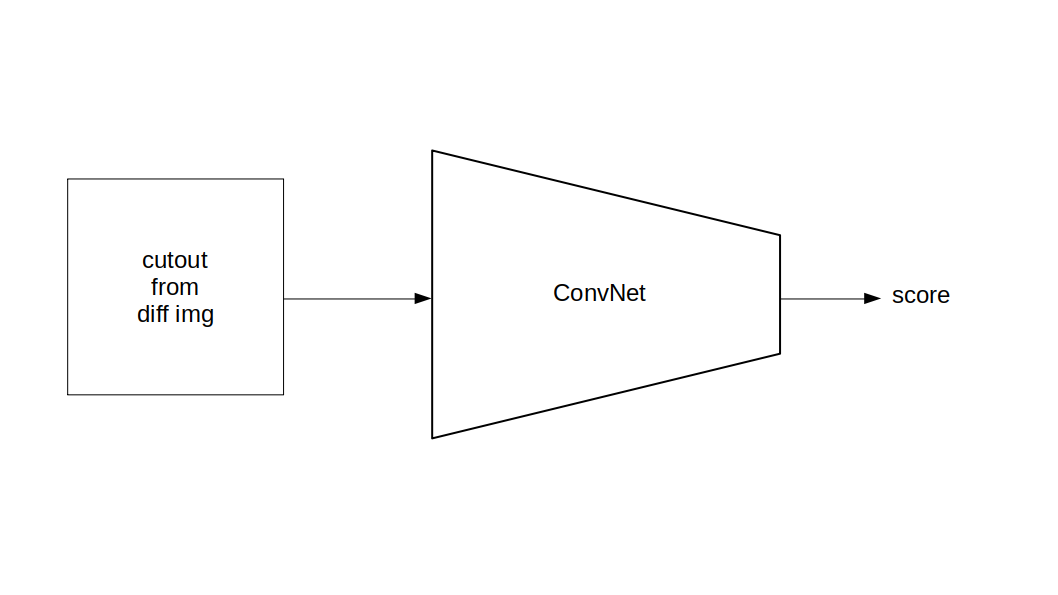
\includegraphics[width=.6\textwidth]{material/rb-classifier}
  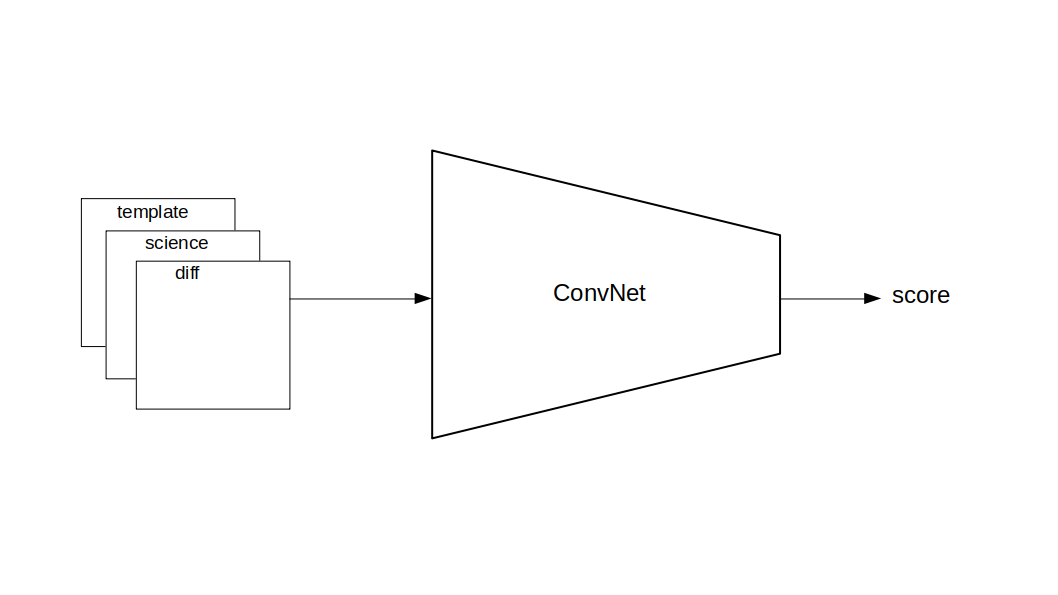
\includegraphics[width=.6\textwidth]{material/rb-classifier-mod}
  \caption{Classical Real/bogus classifier (top) and the modified 3D classifier (bottom)}
  \label{fig:rbdiagram}
\end{figure}

Input-output definition of the problem:
\begin{itemize}
  \item input: cutouts from diff image ($I_d$) with the potential transient at the center
  \item output: reliability score for the potential transient
\end{itemize}

Although the output of a classifier is categorical (i.e. a class label), we will be using the output before the last Softmax~\footnote{TBD} layer, which can be interpreted as a probability or score.

\subsection{The score}
As the task definition embraces a recognition according to spatial \emph{and} temporal features simultaneously, the score needs to be defined carefully to capture both aspects.
More specifically, we need to define the term ``real'' more precisely: a non-astrophysical detection, such as an artifact, is obviously not ``real''. But how about a non-varying astrophysical source?

\begin{figure}[h]
  \centering
  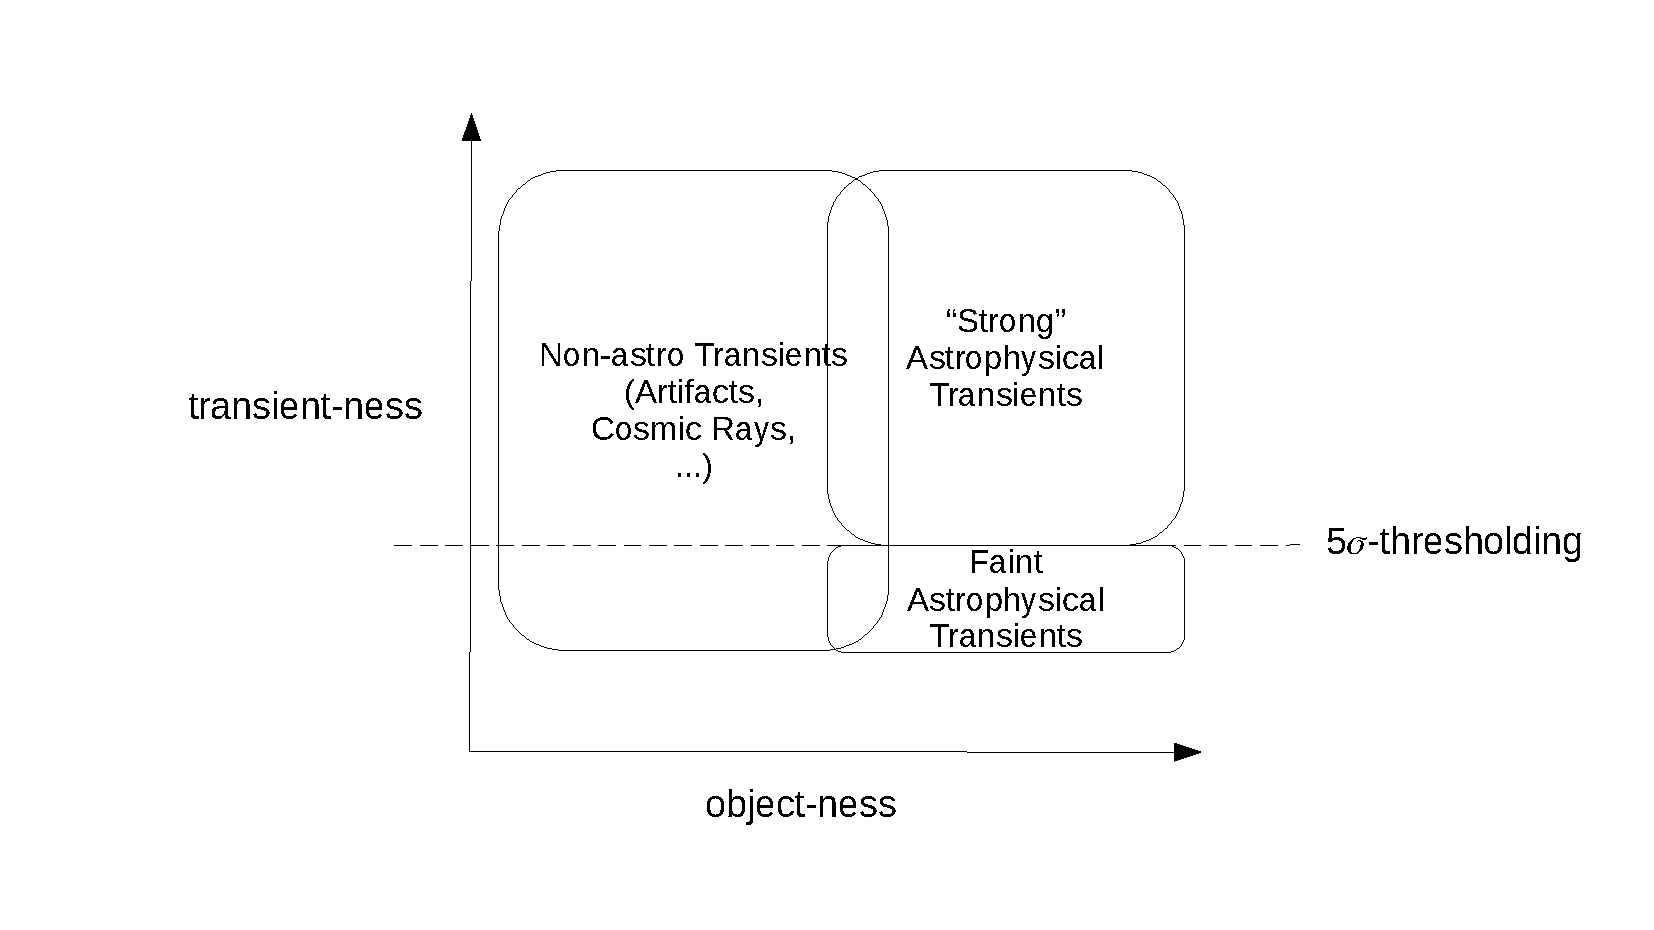
\includegraphics[width=.8\textwidth]{material/score-space}
  \caption{The 2-dimensional realness space}
  \label{fig:score-space}
\end{figure}

As illustrated in figure~\ref{fig:score-space}, the real-ness space is composed of (at least) two dimensions, which we name ``transient-ness'' and ``object-ness''.

There are multiple available options:
\begin{itemize}
\item simple binary classification -- the resulting score may not be quite informative
\item regression -- more difficult to define
\item multi-class classification -- difficult data annotation
\end{itemize}

If we go with regression... there are bogus detections, variables, ``appearing transients''
\begin{equation}
  s=\left| \frac{A_2-A_1}{A_2+A_1} \right|
\end{equation}


\subsection{Drawbacks}
\begin{itemize}
\item has no access to the temporal~\footnote{throughout this document the term ``temporal'' is used to represent the transition from a template/reference image to a science image. It has to do, but should not be confused with the ``real'' time axis!} behavior of the source. This is by definition outsourced to the upstream image differencing module and hence there is no ``learned intelligence'' in processing the ``transient-ness'' of the candidate.
\item any ``miss'' (false negative) in the upstream modules is inherited and irrecoverable.
\item can only handle single object per cutout -- when there are multiple true transients, it \emph{has to} ignore the others.
\end{itemize}

The first two drawbacks are a result of having separated the temporal processing (i.e. image differencing) from the final classification, whereas the last one has to do with how the problem and solution are defined based on cutouts.

% \paragraph{The case of ambiguous negatives}
% As of now it is not quite clear what a ``negative'' is for training; in the broadest implementation it can be cutout that is not positive. But since the inputs to this module are the outputs of imdiff, one could only use ``bogus candidates'' as negatives, which is closer to what happens in practice, and may give better results.


\subsection{Benefits}
\label{sec:rb_benefits}

Although as discussed this is just a sub-optimal learning-based approach to this problem, it still has the advantage of \emph{interpretability}; the generated output might be too contaminated with false alarms and (at the same time) missed true transients, but the process is fully transparent to the downstream users of the alerts and they have the possibility to develop their own post-processing blocks per need.


\subsection{What will be learned?}
Since the temporal behavior of the candidates fed to this module is assumed, it is foreseeable that the neural network will eventually learn a concept close to ``PSF-ness'', true to its title; real/bogus classification.

\subsection{Modified 3D Real/Bogus Classifier}
In this implementation the classifier has access to the template, science image pairs along with the diff image. This allows the network to make use of the temporal behavior of the source too.
Note however that still the difference image has a key role in the process, as the images are cropped around the sources detected in the difference image.

\subsection{End-to-End Simultaneous Localization and Classification (~TransiNet)}

\begin{figure}[h]
  \centering
  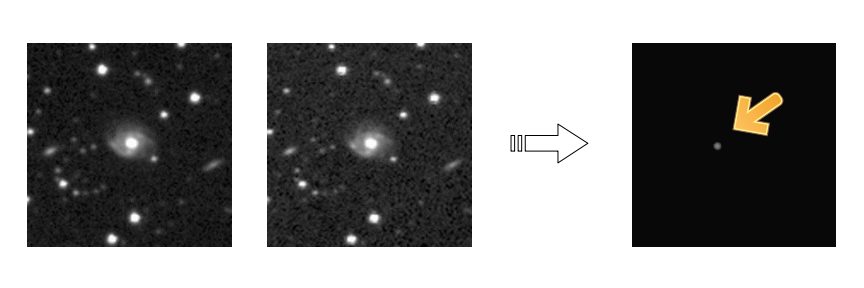
\includegraphics[width=.8\textwidth]{material/transinet-teaser}
  \caption{End-to-end image differencing, localization and classification. The output has to be clean and complete \emph{by definition} }
  \label{fig:transinet-teaser}
\end{figure}

\begin{itemize}
  \item input: a pair of science,template images: $(I_t,I_s)$
  \item output: $S_t$, set of true transients
  \item intermediate output: a ``score image'' where scores are assigned per-pixel
\end{itemize}

Based on TransiNet~\cite{transinet}. Does full detection (localization + classification) simultaneously -- along with any necessary implicit steps.
Since the temporal and spatial behaviors are considered at the same time, the definition of the task of this module would be to find all the time-variable real astronomical sources -- corresponding to the high-level definition of the problem in \ref{sec:definition}.





% \section{Notes from the template}

% \subsection{How to handle LSST standard references?} 

% The papers should cite standard LSST references\footnote{See \url{https://github.com/lsst-pst/LSSTreferences}}, 
% where appropriate. For the usage, please see below.  These examples all use the ADS handle, unless they are 
% project docs then the use the project handle like LSE-17.

% All are on the lsst-texmf which you can get from \url{http://lsst-texmf.lsst.io}


% \subsubsection{LSST System and Science}

% The LSST system (brief overview of telescope, camera and data management subsystems),
% science drivers and science forecasts are described in:

% \begin{itemize}
% \item LSST Science Requirements Document: \cite{LPM-17}.
% \item LSST overview paper: \cite{2008arXiv0805.2366I}.
% \item LSST Science Book: \cite{abell2009lsst}.
% \end{itemize}
% %------------------------------------------------------------------------------


% \subsubsection{Simulations}

% The LSST simulations are described in a series of papers. Use of the LSST simulations should cite the LSST simulations overview paper \cite{2014SPIE.9150E..14C} and the specific simulation tools used:

% \begin{itemize}
% \item LSST Catalogs (CatSim): \cite{2014SPIE.9150E..14C}
% \item Feature-Based Scheduler: \cite{2018arXiv181004815N}
% \item Operations Simulator (OpSim): Scheduler \cite{2016SPIE.9910E..13D}, SOCS \cite{2016SPIE.9911E..25R}
% \item Metrics Analysis Framework (MAF): \cite{2014SPIE.9149E..0BJ}
% \item Image simulations (Phosim): \cite{2015ApJS..218...14P}
% \item Sky brightness model: \cite{2016SPIE.9910E..1AY}
% \item LSST Performance for NEO (or moving object) discovery: \cite{2018Icar..303..181J}
% \end{itemize}
% %------------------------------------------------------------------------------


% \subsubsection{Data Management}

% LSST data management system and the data products are described in:

% \begin{itemize}
%   \item The LSST Data Management System: \cite{2015arXiv151207914J}
%   \item Data Products Definition Document: \cite{LSE-163}
% \end{itemize}
%  %------------------------------------------------------------------------------


% \subsubsection{Camera}

% \begin{itemize}
%    \item Design and development of the LSST camera: \cite{2010SPIE.7735E..0JK}
% \end{itemize}
% %------------------------------------------------------------------------------


% \subsubsection{Telescope and Site}

% \begin{itemize}
%    \item Telescope and site overview and status in 2014:  \cite{2014SPIE.9145E..1AG}
% \end{itemize}
% %------------------------------------------------------------------------------

% \subsubsection{System Engineering}

% \begin{itemize}
%    \item LSST systems engineering: \cite{2014SPIE.9150E..0MC}
%    \item System verification and validation: \cite{2014SPIE.9150E..0NS}
% \end{itemize}
% %


